\section{Homography and Visual Object Tracking}
\label{sec:HomographyAndVisualObjectTracking}

This section is dedicated to one of our experiments that were not completely related to the \gls{vot} itself, yet we achieved an original scientific contribution in this area when exploring certain solutions that could be applicable to object tracking, especially traffic analysis. Even though we did not set out for homography-based object tracking (explained later) due to limitations of available datasets, still we would like to elaborate on our developed approach. The proposed method was fully described as well as scrupulously tested under difficult conditions. We wrote up the whole research process in a paper called \textbf{Homography Ranking Based on Multiple Groups of Point Correspondences}~\cite{ondrasovic2021homography}, published in journal \textbf{Sensors} (web:~\cite{sensors}), under the category \emph{Physical Sensors}. In what follows, we provide a concise report of our research. For more information, we suggest the reader use our aforementioned article. Moreover, our preliminary discussion of this possibility with initial proposal of the solution can be found in our first paper dubbed \textbf{Foundations for homography estimation in presence of redundant point correspondencies}~\cite{ondravsovivc2020foundations} published in \textbf{Mathematics in Science and Technologies} (web:~\cite{mistconf}) conference.

\subsection{General Introduction}

One of the fundamental tasks of computer vision is to deal with various image transformations that may improve the outcome of subsequent post-processing phase. One transformation that was of particular interest to our goal of traffic analyis is the perspective transformation. More concretely, a removal of perspective distortion. To achieve this, the so-called homography mapping is often exploited.

Homography is a perspective projection of a plane from one camera view into a different camera view. The perspective projection maps points from a $3$D world onto a $2$D image plane along lines that emanate from a single point~\cite{geetha2013automatic, bousaid2020perspective}. This projection is performed by a $3 \times 3$ invertible transformation matrix called the homography matrix (or just homography) with $8$ \gls{dof}. A general homography matrix may be defined as
\begin{equation}
    \label{eq:HomographyMatrix}
    \H =
    \begin{bmatrix}
        h_{11} & h_{12} & h_{13}\\
        h_{21} & h_{22} & h_{23}\\
        h_{31} & h_{32} & h_{33}
    \end{bmatrix}
\end{equation}
This transformation is used to achieve the mapping between two views of the same plane, since in the pinhole camera model, any two images of the same planar surface are related to each other by the homography~\cite{hartley2003multiple, hartley1997defense}. More specifically, a single vector $\vectt{u}{u_x, u_y, 1}$, representing a warped keypoint in homogeneous coordinates, is mapped onto the rectified keypoint  $\vectt{\tilde{u}}{\tilde{u}_x, \tilde{u}_y, 1}$ by the homography $\H$ using the transformation $s \vect{\tilde{u}} \approx \H \vect{u}$, with $s$ being the scale factor. In its most general form, homography may achieve mapping between various perspectives. However, for our purposes we focused only on producing a view where perspective distortion is absent, i.e., to rectify the image so that it looks as if the camera was in an orthogonal position with respect to the desired plane in the world when taking the picture.

Homography is commonly used for rectification of text document images by generating a fronto-parallel view~\cite{lu2005perspective, miao2006perspective}, image stitching~\cite{adel2014image, gao2011constructing}, video stabilization~\cite{liu2015smooth}, extracting metric information from $2$D images~\cite{zhang2000flexible}, pose estimation~\cite{circularmarkerposeestim}, and for various traffic-related applications, e.g., ground-plane detection~\cite{arrospide2010homography}, and bird's-eye view projection~\cite{luo2010low}.

\subsection{Motivation}

The primary motivation to explore the possibility of employing homography for visual object tracking was the fact that as long as a static camera is used and few assumptions that we will discuss later hold, the scene may be easily stripped off the effect of the perspective distoriton. Considering this, the incentive to track vehicles visually using a static camera while exploiting a fronto-parallel view over the road seemed like a plausible extension with possible advantages for traffic analysis. The combination of homography and object tracking is present in the literature, e.g.~\cite{Bose04groundplane, Zhang2012, Mei2009}. To provide more detail, Bose et al.~\cite{Bose04groundplane} presented a fully automated technique for both affine and metric rectification of a given ground plane (up to a scale factor) by simply tracking moving objects. The derivation of the necessary constraints for projective transformation between the image and the ground plane was obtained by observing objects that moved at constant velocity in the world for some part of their trajectory. We conjectured that the extra information about the scene geometry that we may achieve using rectification could aid in making the tracking more accurate. Visual trackers are often supported by motion models such as Kalman filter~\cite{Kalman1960}, so the rationale was to estimate motion model in a orthogonal projection, rather than perspectively distorted one.

\begin{figure}[t]
    \centerline{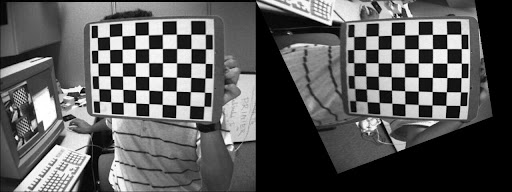
\includegraphics[width=\linewidth]{figures/methodology/chessboard_marker.jpg}}
    \caption[Chessboard marker]{An example of a chessboard marker present in a scene that may be used to establish a point correspondence that may serve for a homography transformation. The rectified, fronto-parallel view demonstrates a desired effect that points present on the ``ground'' plane (in this case, the chessboard) are properly projected, whereas other points suffer from substantial distortion.}
    \label{fig:ChessboardMarker}
\end{figure}

\begin{figure}[t]
    \centerline{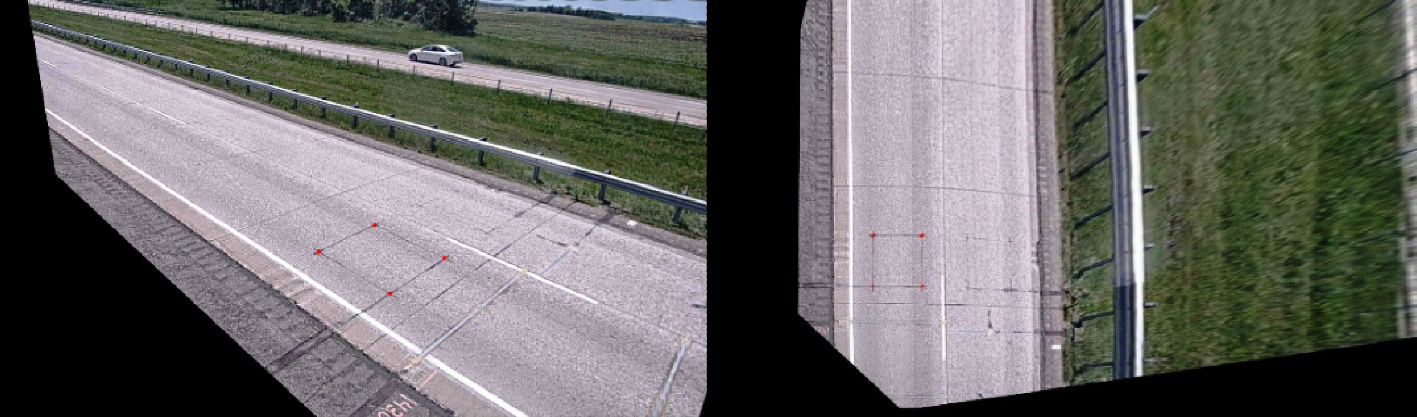
\includegraphics[width=\linewidth]{figures/methodology/homography_road.png}}
    \caption[Square marker on a road]{An example of a virtual square marker present on a road that may be used to establish a point correspondence, and thus the homography transformation, too. The obtained view allows for many applications such as speed and size measurements that would otherwise be a lot more problematic in a perspectively deformed view.}
    \label{fig:RoadMarker}
\end{figure}

A common approach to estimate the homography is to use a set of at least four $2$D point correspondences~\cite{hartley1997defense}. We refer to the points used for establishing the $2$D point correspondences as keypoints. These keypoints may belong to a marker which is an object with a known shape that is either naturally occurring or artificially positioned in the scene. A regular pattern like a chessboard is usually utilized~\cite{zhang2016flexible} (see Fig.~\ref{fig:ChessboardMarker}). A single marker is identified in the image by multiple independent keypoints that have a direct correspondence to its real shape, thus making a group of point correspondences. For the sakes of traffic analysis, the marker may be represented by virtually any points on the image as long as certain conditions are met (see Fig.~\ref{fig:RoadMarker}). However, point correspondences established this way are often noisy and they can introduce errors in the homography estimation. Although $4$ keypoints are satisfactory, often a greater number of keypoints is used, allowing to use optimization to minimize a suitable cost function~\cite{osuna2016multiobjective, mou2013robust}. Then, outlier removal becomes an important step, and algorithms such as RANSAC~\cite{fischler1981random} are usually employed~\cite{osuna2016multiobjective}.

\begin{figure}[t]
    \centerline{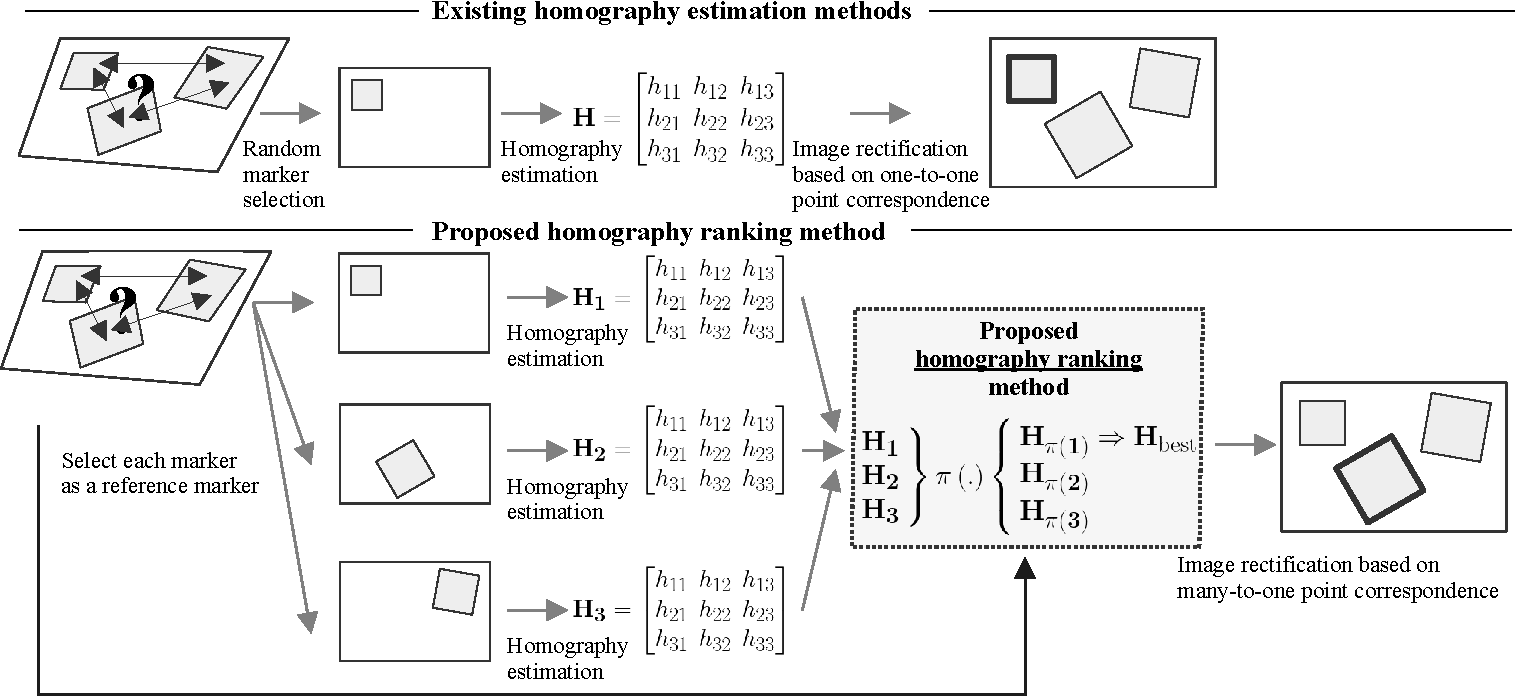
\includegraphics[width=\linewidth]{figures/methodology/homography_motivation_diagram.pdf}}
    \caption[Homography ranking motivation diagram]{Difference between existing homography estimation methods and the proposed homography ranking method. In presence of multiple markers without information about their relative positions in the world, existing approaches can only estimate isolated homographies without the ability to select the best one. Our method extends existing approaches by exploiting multiple markers to rank the isolated homographies.}
    \label{fig:HomographyMotivationDiagram}
\end{figure}

Let us now describe the underlying incentive for developing our approach. Assume a presence of a sole marker in the scene (Fig.~\ref{fig:RoadMarker}). Even though the marker is distorted under perspective, the knowledge of its real shape makes it possible to compute the homography. When multiple copies of the same marker are visible, but their positions in the world are unknown, the knowledge of the shape is not enough to incorporate all the keypoints in the estimation. In the absence of position information, existing approaches for homography estimation based on point correspondences fail because the projection has to preserve the proportional positions. Thus, estimating the homography without knowing the ground-truth layout of the keypoints up to an arbitrary scale does not guarantee the correct result.

Under the aforementioned constraints, existing methods can only generate an isolated homography for each marker based on the one-to-one point correspondence (see Fig.~\ref{fig:HomographyMotivationDiagram}). Each homography may be affected by different sources of noise, e.g., low resolution, blur, or keypoint detection. Thus, the outcome of rectification may vary. Additionally, in many practical applications, a single marker usually covers a small portion of the image which increases susceptibility to noise. The trivial solution would be to use a bigger marker that covers the majority of the estimated plane in the image. However, this solution is often impractical. Furthermore, it is not possible to simply ``merge'' multiple isolated homographies together.

\begin{figure}[t]
    \centerline{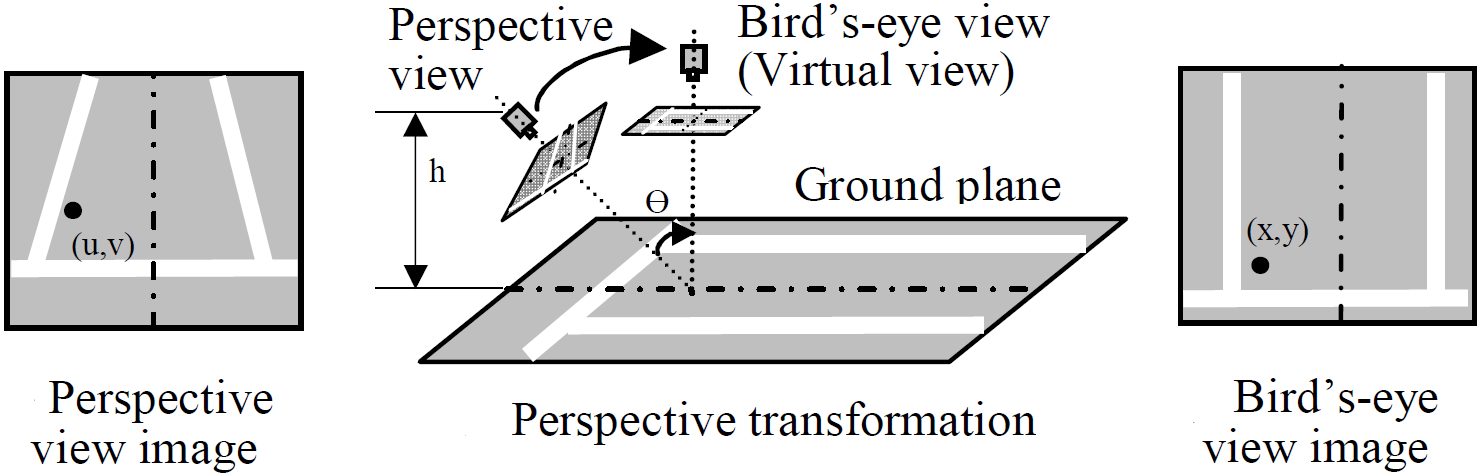
\includegraphics[width=0.7\linewidth]{figures/methodology/road_rectification.png}}
    \caption[Road rectification]{A demonstration of the rectification process when obtaining a fronto-parallel view over the road using homography. \externalsrc{\cite{Luo2010}}}
    \label{fig:RoadRectification}
\end{figure}

\begin{figure}[t]
    \centerline{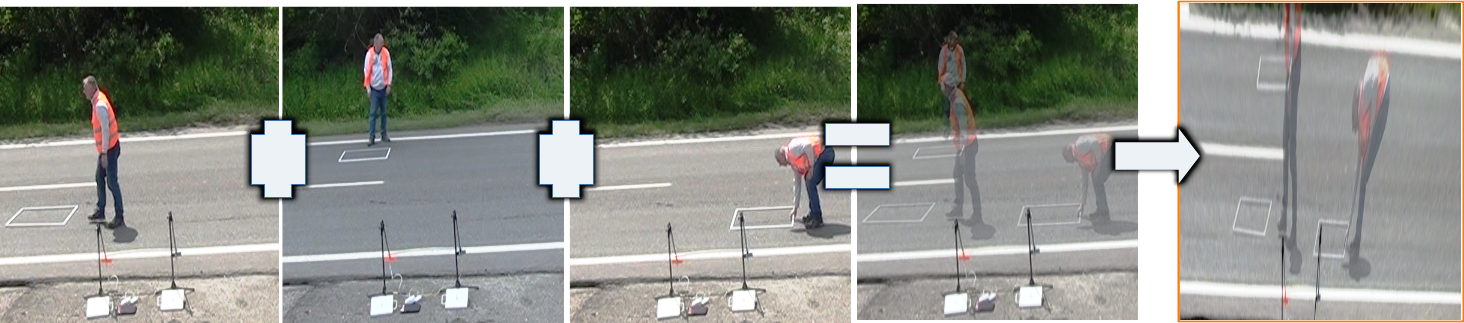
\includegraphics[width=\linewidth]{figures/methodology/markers_on_the_road.png}}
    \caption[Multiple markers on the road]{A motivating real-world example for the proposed method. We can see different frames captured during a video recording that show various positions of the same marker. The picture after the ``equality'' sign is a merge of the previous frames for better illustration. Due to the use of a static camera, we may treat positions of the given marker on individual frames as if they were captured simultaneously. However, the question still remains unanswered. Given multiple markers in the absence of their position information, which one is the best to choose for rectification?}
    \label{fig:MultipleMarkersOnRoad}
\end{figure}

This work was motivated by a real-world application of generating a bird's-eye view over a road (see Fig.~\ref{fig:RoadRectification}) from a video recording when we could not use a large marker to cover a sufficient portion of the road (see Fig.~\ref{fig:MultipleMarkersOnRoad}). Homography estimation based on a single small marker was inaccurate. Therefore, we tried to use multiple small markers and measure their relative positions. However, their position measurements were highly noisy at best. Thus, the proposed method was used, instead. It is important to note that our method can also be adopted in a situation when the marker placed at various positions on the same planar surface is visible at different frames using a static camera. Stacking the frames onto each other yields a view with multiple markers.

\subsection{Developed Method}

The proposed method is based on the following assumptions:
\begin{enumerate}
    \item The markers are geometrically similar, i.e., they differ only in translation, rotation, and uniform scale in the real world.
    \item The shape of at least one of them is known.
    \item These markers are placed on the same planar surface in the scene.
\end{enumerate}
Our approach shows a way to relate all the markers to each other in a single score function without knowing their relative positions in the scene. Our method only handles transformation from a distorted to the undistorted view of the target plane. Thus, it serves for the removal of perspective distortion only.

We exploited the properties of homography and similarity transformations and expressed them in a single score function. This function stands at the core of our contribution. Its value is used as a proxy to rank homographies according to their reprojection error over the entire image using only markers' keypoints. The usual use case would be to select the homography with the lowest score, i.e., the highest-ranked matrix, to perform the image rectification.

\begin{figure}[t]
    \centerline{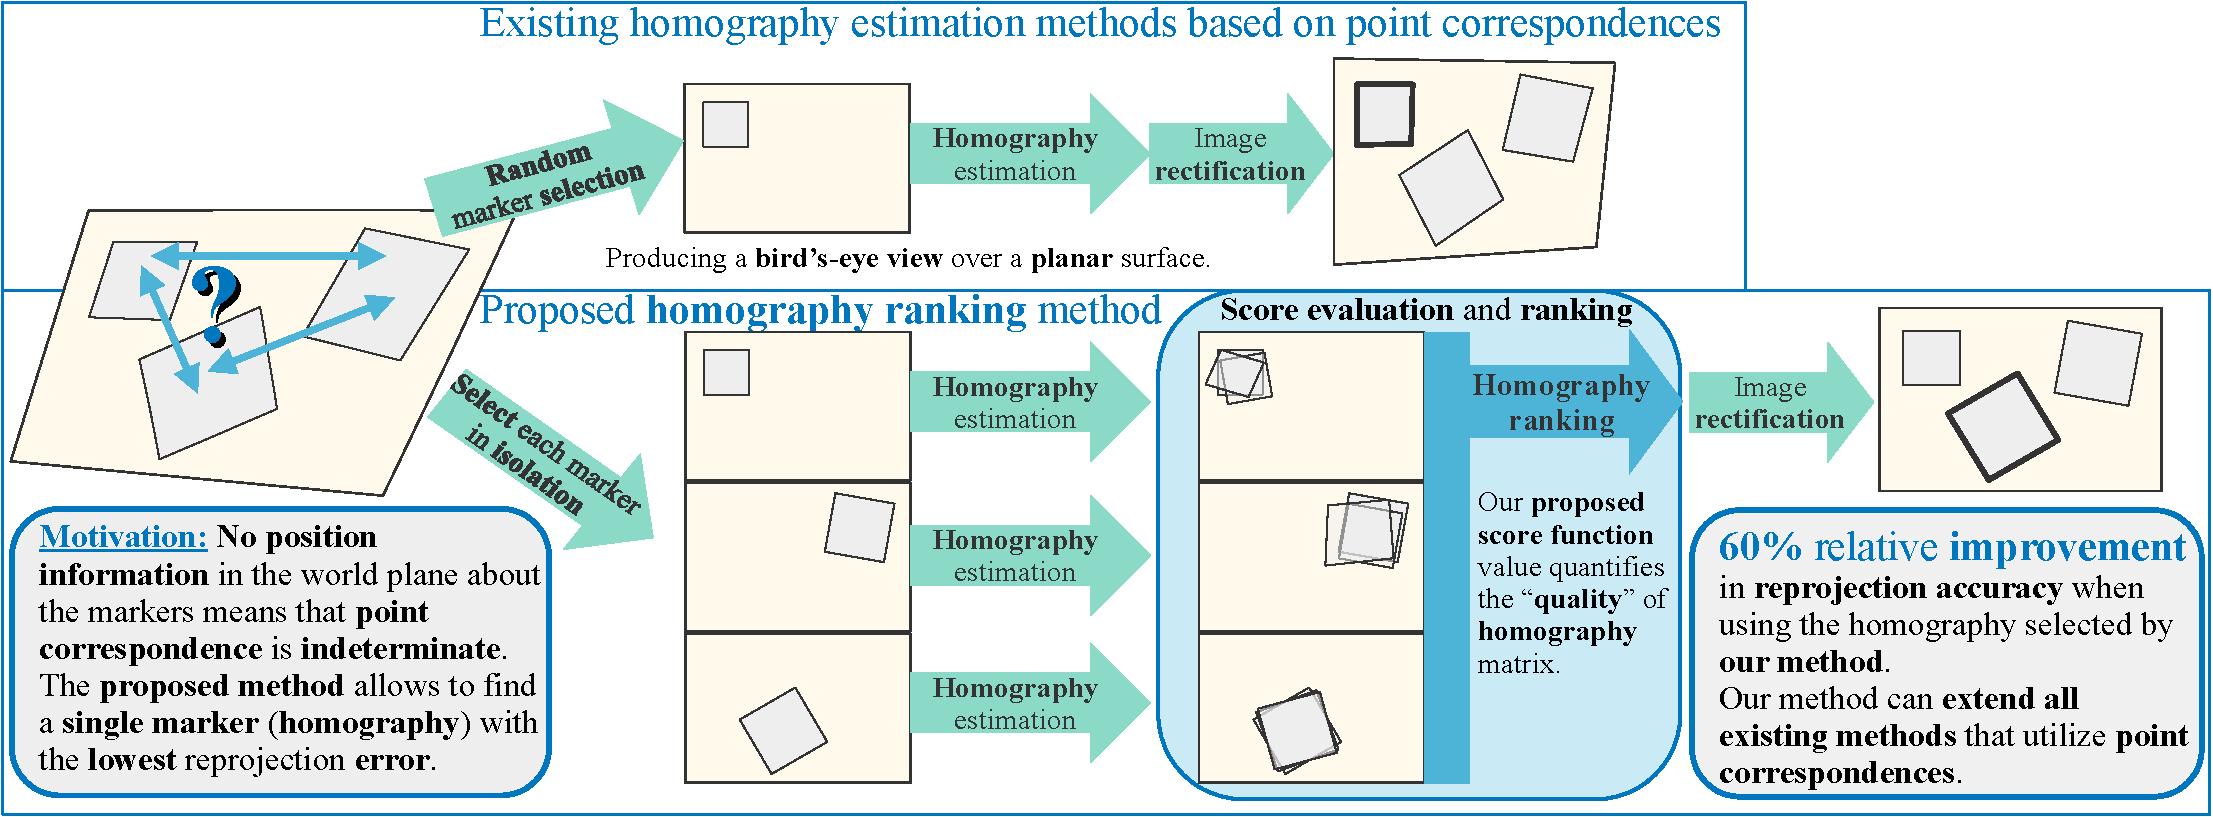
\includegraphics[width=\linewidth]{figures/methodology/graphical_abstract.pdf}}
    \caption[Homography ranking graphical abstract]{Here we present the graphical abstract from our paper. The basic idea is that existing approaches may only estimate an isolated homography for each marker and cannot determine which homography achieves the best reprojection over the entire image. Therefore, we proposed a method to rank isolated homographies obtained from multiple distinct markers to select the best homography. This method extends existing approaches in the post-processing stage, provided that the point correspondences are available and the markers differ only by similarity transformation after rectification. We demonstrated the robustness of our method using a synthetic dataset and showed an approximately $60\%$ relative improvement over the random selection strategy based on the homography estimation from the OpenCV library.}
    \label{fig:GraphicalAbstract}
\end{figure}

\begin{figure}[t]
    \centerline{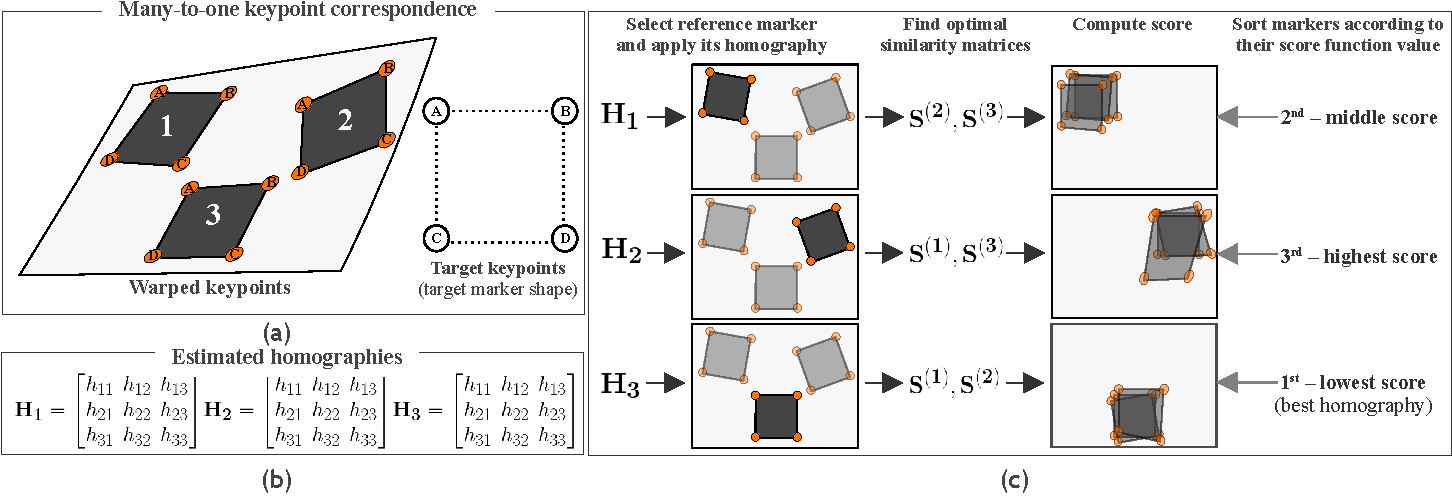
\includegraphics[width=\linewidth]{figures/methodology/system_diagram.pdf}}
    \caption[Homography ranking system diagram]{A system diagram describing the general idea behind our method. \textbf{(a)} The input consists of a many-to-one point correspondence specified by geometrically similar markers and information about the shape of the target marker. \textbf{(b)} We assume that the isolated homographies corresponding to each independent marker are provided on the input as well. \textbf{(c)} The algorithm processes each marker by applying its homography matrix to the image to produce a rectified image. Subsequently, it computes optimal similarity matrices corresponding to the auxiliary markers. The computation of the score function makes use of these transformations. The obtained score values then serve for comparison to rank (sort in ascending order) the homographies. The homography ranked first is considered the ``best'' candidate for the minimal reprojection error over the entire image.}
    \label{fig:HeatmapsBestWorst}
\end{figure}

Our algorithm is invariant to the underlying homography estimation method. It can thus serve as an extension to approaches that handle point correspondences, either as part of run time or a post-processing stage. Moreover, it is computationally very efficient, as it scales well with a quadratic complexity $\func{\Theta}{m^2}$.

\subsection{Experiments and Discussion}

Fig.~\ref{fig:HeatmapsBestWorst} shows how the reprojection error varies with respect to the marker position. We can see that the marker position can be deduced by looking at the heatmap representing the pixel-wise reprojection error over the image. The transformation achieves the best accuracy in the marker neighborhood and steadily decreases for more distant pixels. However, not all markers are subjected to the same pattern of error variation. This observation was the core motivation for our solution. We aim to choose the marker that minimizes the pixel-wise reprojection error within the region of the image that is as broad as possible. That is why we evaluate our method by computing the reprojection error over each pixel, not just the keypoints.

\begin{figure}[t]
    \centerline{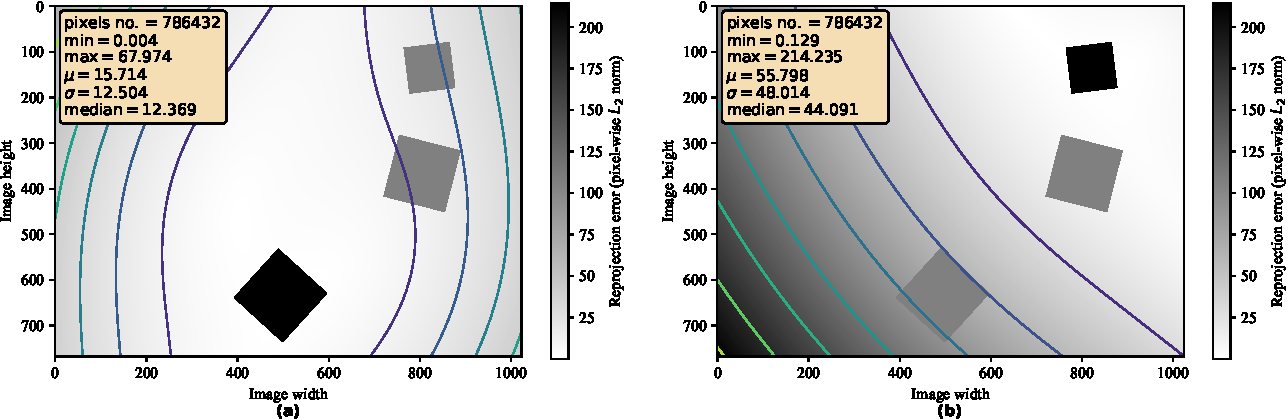
\includegraphics[width=\linewidth]{figures/methodology/heatmaps_best_worst.pdf}}
    \caption[Homography ranking heatmaps]{Distribution of pixel-wise reprojection error. The heat map together with corresponding contours demonstrate the varying distance between the ground truth and rectified pixel position after removing the perspective distortion. The bold square represents the reference marker. We show the result of \textbf{(a)} the ``best'' marker and \textbf{(b)} the ``worst'' marker. This test scenario includes all similarity transformations as well as noise in point correspondence.}
    \label{fig:HeatmapsBestWorst}
\end{figure}

We evaluated the proposed homography ranking algorithm in various conditions. We tested cases involving various similarity transformations applied to original markers as well as noisy point correspondence, e.g., errors in marker detection since these are the expected problems in real-world scenarios.

We demonstrated that the proposed solution is robust in presence of noise in the point correspondences. These correspondences can be either algorithmically found using feature-matching algorithms (e.g., SIFT~\cite{lowe1999object}, SURF~\cite{bay2008speeded}) or annotated manually. But even human annotations are often inaccurate. We also showed the robustness of our method to a varying number of markers and a change in shape.

All our test scenarios demonstrated the following trend. On average, the homography with the highest score improved the relative performance to the baseline performance the most (both median and mean above $60$\%). The lowest-ranked homography often led to a lot worse performance (median and mean around $-90$\%). These values varied slightly across different setups. The shape and number of markers had the greatest influence. All the improvements in between steadily decreased, reached $0$\% improvement at around $\nicefrac{2}{3}~m$, where $m$ is the number of markers. A general claim is that the first half of ranked homographies yields a better reprojection compared to the baseline on average. The baseline performance was given by an average OpenCV~\cite{bradski2008learning} reprojection error under the assumption of no prior preference of specific markers, hence the random marker selection.
